% LaTeX Article Template
\documentclass[11pt,a4paper,oneside]{article}
\usepackage{amsmath,amsxtra,amssymb,latexsym, amscd,amsthm}
\usepackage{graphicx}
\usepackage{indentfirst}
\usepackage[mathscr]{eucal}
\usepackage[utf8]{vietnam}
\usepackage{graphicx}
\usepackage{fullpage}
\usepackage{multirow}
\usepackage{rotating}
\graphicspath{{./images/}}
\newtheorem{modeling_def}{Định nghĩa }
\DeclareGraphicsExtensions{.jpg,.png,.pdf}
\begin{document}

\title{Toán học rời rạc dành cho các nhân viên kiểm thử}         % Ten bai
\author{
Trần Văn Mạnh, Bùi Hoàng Khánh\\
Lớp K16-CNPM3, trường ĐHCN, Đại học quốc gia Hà Nội
}        % Tac gia
\date{}         % Ngay
\maketitle
\begin{abstract}
Toán rời rạc là một lĩnh vực quan trọng trong tin học, để hiểu nó một cách thấu đáo vả sâu sắc quả thật không đơn giản. Bài viết này chỉ tập trung vào nghiên cứu toán rời rạc dành cho các nhân viên kiểm thử phần mềm. Các nhân viên kiểm thử phần mềm coi Toán rời rạc như một công cụ giúp học có được tư duy logic chặt chẽ hơn trong quá trình kiểm thử phần mềm để tránh bỏ xót những lỗi không đáng tiếc.
Trong tâm của bài viết này đi vào nhiên cứu các khái niệm cơ bản như lý thuyết tập hợp, các hàm, các mối quan hệ, logic mệnh đề, lý thuyết xác suất.\\
Phần lý thuyết tập hợp chúng tôi trình bày các khái niệm như định nghĩa tập hợp, tập rỗng, biểu diễn tập hợp bởi biểu đồ Venn. Các phép toán trên tập hợp, mối quan hệ giữa các tập hợp. Phân hoạch một tập hợp thành các tập con và các phép toán đồng nhất thức giữa các tập hợp. \\
Phần các hàm chung tôi trình bày các khái niệm liên quan đến miền và phạm vi. Các loại hàm và luật hợp thành hàm. 
Phần các quan hệ trình bày các quan hệ liên quan đến tập hợp và các quan hệ liên quan đến một tập đơn.
Phần logic mệnh đề trình bày các khái niệm các toán tử logic, biểu thức logic và các quan hệ tương đương.
Phần lý thuyết xác suất trình bầy một số khái niệm như định nghĩa và một số cách sử dụng lý thuyết xắc suất trong vấn đề kiểm tra bộ test case có đảm bảo hết được các chức năng cần thiết khi kiểm thử một phần mềm.\\
Nói chung trong mỗi phần chúng tối đều đưa nhưng mình họa ví dụ cụ thể việc ứng dụng cho nó trong kiểm chứng phần mềm như thế nào.
Phần cuối chúng tôi trình bày vị thế của toán rời rạc trong các kỹ thuật kiểm thử phần mềm. Phần này chỉ muốn làm rõ thêm là toán rời rạc được ứng dụng rất nhiều trong các kỹ thuật kiểm thử chức năng. 
Chúng tôi hy vọng sẽ phần nào chuyển tải được những gì mình đã nghiên cứu và tìm hiểu đến bạn đọc. 
\\

\textit{
Lời chú của các học viên Trần Văn Mạnh, Bùi Hoàng Khánh:\\
Những nội dung trình bày trong bài viết này phần lớn dựa trên chương 3, cuốn sách ``Software testing - a Craftman's approach, second edition'' của tiến sỹ Paul C.Jorgensen, Department of Computer science and Information Systems, Grand Valley State University\\
Khả năng của chúng tôi là có hạn và chưa đủ để nghiên cứu một đề tài lớn như trong sách này. Do vậy chúng tôi cố gắng đọc hiểu, tham khảo các tải liệu, và truyền tải lại nội dung dưới dạng một bài báo. Tuy nhiên bản quyền nội dung vẫn hoàn toàn là của tác giả Tiến sỹ Paul C.Jorgensen.
} 
\end{abstract}

\section{Giới thiệu chung}       % Muc dau tien
Từ trước đến nay khi nói đến IT người ta thường nghĩ ngay đến những chuyên gia về bảo mật dữ liệu, chuyên gia quản trị dự án và chuyên gia phần mềm. Ít ai nhắc đến chuyên gia đảm bảm bảo chất lượng phần mềm. Một phần cũng do người trong giới IT cũng như ngoại đạo chưa đánh giá được đúng bản chất của kiểm thử và đảm bảo chất lượng phần mềm. Phần nữa là dường như những năm trước đây ngay ở các trường đại học cũng chưa thật coi trọng vấn đề này khi đưa vào giáo trình giảng dạy ở các bậc đại học cũng như sau đại học. Tuy nhiên những năm gần đây, do tốc độ phát triển như vũ bão của ngành công nghệ thông tin. Các phần mềm hiện nay lớn hơn rất nhiều về khối lượng cũng như độ phức tạp về mặt nghiệp vụ. Cho nên vấn đề đảm bảo phần mềm chạy đúng và không có lỗi cũng như chất lượng tốt đã ngày càng trở lên quan trọng. Và trong công nghệ phần mềm bộ phận quản lý chất lượng phần mềm trở lên hết sức quan trọng, một trong những đội ngũ của họ là những nhân viên kiểm thử. Họ là những người làm nhiệm vụ để phần mềm luôn luôn chạy đúng và tối ưu ở mức chấp nhận được. Vậy căn cứ vào đâu, tiêu chí nào và nền tảng vững chắc gì để có thể một trở thành một nhân viên kiểm thử chuyên nghiệp. Đó chính là họ cần có nền tảng toán học vững chắc, đặc biệt là toán rời rạc. Nó sẽ giúp ích rất nhiều cho công việc sau này của họ. Vậy sẽ có người tự hỏi, toán rời rạc giúp ích gì cho các nhiên viên kiểm thử. Để trả lời câu hỏi này chúng ta sẽ nghiên cứu từng bước một về các khái niệm như lý thuyết tập hợp, các hàm, các mối quan hệ, logic mệnh đề, lý thuyết xác suất, mỗi trong số đó sẽ được thảo luận ở đây.
\section{Lý thuyết tập hợp} 

Thật là boăn khoăn khi chấp nhận rằng không tồn tại một định nghĩa cụ thể nào về tập hợp. Điều này thật sự là một phiền toái bởi vì lý thuyết tập hợp là trọng tâm của 2 chương toán học này. Theo đó, lý thuyết toán học đã đưa ra một sư phân loại quan trọng, lý thuyết tập hợp sơ khai và lý thuyết tập hợp tiên đề (axiomatic). Trong tập hợp sơ khai (naive), một tập hợp được coi như một số hạng nguyên thủy (Primitive term), nó giống như điểm và điểm dòng và dòng là các khái niệm nguyên thủy trong hình học. Có một số từ đồng nghĩa với tập hợp như: bộ sưu tập, nhóm, chum. Bạn đã hiểu ý ở đây. Một điều quan trọng về tập hợp là nó cho phép chúng ta quy một vài thứ thành một nhóm hay toàn bộ . Ví dụ, chúng ta muốn quy một tập hợp các tháng, mà có chính xác 30 ngày. (Chúng ta cần nhớ tập hợp này khi chúng ta kiểm thử chức năng NextDate trong chương 2). Trong lý thuyết tập hợp chúng ta viết:

\begin{center}
M1 = $\{$April,  June,  September, November$\}$\\
\end{center}
và chúng ta đọc ký hiệu này là “M1 là một tập hợp gồm các phần tử là các tháng April, June, September, November.”
\subsection{Các thành phần của tập hợp}
Các đối tượng trong một tập hợp được gọi là các thành phần của một tập hợp, và mối quan hệ này được miêu tả bằng biểu tượng “thuộc”, do đó chúng ta có thể viết April thuộc M1. Khi một đối tượng nào đó không là thành phần của tập hợp, chúng ta sử dụng biểu tượng “không thuộc”, chúng ta có thể nói December không thuộc M1.

\subsection{Định nghĩa tập hợp}
Một tập hợp được định nghĩa theo ba cách: bằng cách liệt kê các phần tử của nó, bằng cách đưa ra một quy tắc quyết định hoặc bằng cách xây dựng tập hợp từ các tập hợp khác. Phương án liệt kê các phần tử được sử dụng trong trường hợp các tập hợp chỉ có ít phần tử cũng như trong các tập hợp mà các phần tử của nó tuân theo một kiểu mẫu rõ ràng. Chúng ta có thể xác định một tập hợp các năm trong chương trình Nextdate như sau:
\begin{center}
Y = $\{$1812, 1813, 1814,\ldots, 2011, 2012$\}$\\
\end{center}
Khi định nghĩa một tập hợp bằng cách liệt kê các phần tử của nó, trật tự của các phần tử sẽ không quan trọng. Chúng ta hiểu lý do tại sao khi chúng ta thảo luận về đẳng thức tập hợp (set equality). Phương pháp quy tắc quyết định (Decision rule approach) thì phức tạp hơn, và sự phức tạp này mang lại cả lợi ích và bất lợi. Chúng ta có thể định nghĩa các năm cho NextDate như sau:
\begin{center}
Y = $\{$year :  1812 \leq year \leq 2012$\}$\\
\end{center}
Chúng ta đọc “Y là tập hợp các năm sao cho các năm từ 1812 đến 2012”. Khi một quy tắc quyết định được dùng để định nghĩa một tập hợp, quy tắc đó phải rõ ràng. Do đó, khi được đưa gia bất cứ giá trị hợp lý nào của năm, chúng ta có thể quyết định liệu năm đó có thể thuộc tập hợp Y hay không. Lợi ích của phương pháp định nghĩa tập hợp bằng các quy tắc quyết định là yêu cầu về sự rõ ràng của nó tạo ra tính rõ ràng. Các Testers có kinh nghiệm đã gặp phải rất nhiều yêu cầu không thể được kiểm thử. Trong nhiều lần, lý do về các yêu cầu không được kiểm thử dẫn đến một quy tắc quyết định rõ ràng. Trong chương trình hình tam giác của chúng ta là một ví dụ, giả sử chúng ta định nghĩa một tập hợp:
\begin{center}
N = $\{$t: là một tam giác có các cạnh gần bằng nhau$\}$\\
\end{center}
Chúng ta có thể nói rằng, tam giác với các cạnh (500, 500, 501) là 1 phần tử của N , nhưng chúng ta sẽ làm thế nào với những tam giác có các cạnh là  (50, 50, 51) hay (5, 5, 6)?

Điểm lợi thứ hai của phương pháp định nghĩa tập hợp bằng các quy tắc quyết đinh là chúng ta có thể gặp khó khăn, ví dụ chúng ta có thể quan tâm đến tập hợp:
\begin{center}
S = $\{$Bán hàng : 15\% tỉ lệ hoa hồng áp dụng tới việc bán hàng$\}$\\
\end{center}
Chúng ta không dễ dàng viết ra các phần tử của tập hợp này, nhưng được cho một giá trị đặc biệt cho bán hàng, chúng ta có thể dễ dàng áp dụng quy tắc quyết định. Bất lợi chính của các quy tắc quyết định là ở chỗ chúng có thể trở nên phức tạp một cách hợp lý, đặc biệt khi chúng ta được trình bày các biểu thức với các phép toán tồn tại và với mọi cho tất cả. Nếu mọi người hiểu các ký hiệu này, chính xác là hữu ích: rất thường xuyên, các khách hàng bị căng thẳng bởi các báo cáo với các lượng tử hóa. Một vấn đề thứ hai với nguyên tắc quyết định đã làm với chính tài liệu tham khảo. Điều này thật thú vị , nhưng nó thật sự ứng dụng rất ít cho testers. Vấn đề phát sinh khi một quy tắc quyết định liên quan đến bản thân, mà là một chu kỳ (circularity). Ví dụ Barber của Seville (trong truyện cổ tích hay ngụ ngôn gì đó) “là người đàn ông cạo tất cả những người không cạo mình.”

\subsection{Tập rỗng}
Tập hợp rỗng, được ký hiệu là {\O}, chiếm một vị trí đặc biệt trong lý thuyết tập hợp. Tập hợp rỗng không chứa phần tử nào. Về điểm này, các nhà toán học đã sẽ lạc đề khi chứng minh các cơ sở lập luận về các tập hợp rỗng:
\begin{itemize}
\item Tập hợp rỗng là duy nhất, điều đó có nghĩa là, sẽ không có hai tập hợp rỗng.
\item ${\O}, \left\{{\O}\right\}, \left\{\left\{{\O}\right\}\right\}$,  là những tập hợp khác nhau.  \\
\end{itemize}
Rất hữu ích để chú ý rằng, khi một tập hợp được định nghĩa theo một nguyên tắc quyết định điều đó  luôn luôn sai, thì tập hợp đó là tập hợp rỗng. Ví dụ:
\begin{center}
{\O} = $\{$year :  2012 \leq year \leq 1812$\}$\\
\end{center}

\subsection{Các biểu đồ Venn}
Tập hợp thường được mô tả bằng các biểu đồ Venn, như trong chương 1, khi chúng ta thảo luẩn về các tập hợp các hành vi cụ thể và các hành vi được lập trình. Trong một biểu đồ Venn, một tập hợp được mô tả là các điểm hình tròn, trong của một vòng tròn chứa các phần tử của một tập hợp. Sau đó, chúng ta có thể vẽ tập hợp M1 gồm các tháng có 30 ngày ( hình \ref{fig:mtran_ima1}).

\begin{figure}
\setlength\fboxsep{1mm}
\setlength\fboxrule{1pt}
\begin{center}
\fbox{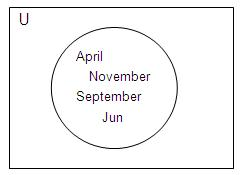
\includegraphics[width=7.5cm,keepaspectratio]{mtran_ima1}}
\caption{Biểu đồ Venn của tập hợp gồm những tháng 30 ngày}
\label{fig:mtran_ima1}
\end{center}
\end{figure}
Các biểu đồ Venn cho ta biết có nhiều mối quan hệ tập hợp khác nhau một cách trực quan, nhưng một số có vẻ cầu kỳ được đặt ra. Các tập hợp vô hạn khác hữu hạn (Infinite and finite sets) như thế nào? Cả hai loại này có thể được biểu diễn trong biểu đồ Venn, trong trường hợp các tập hợp hữu hạn, chúng ta giả định rằng mỗi điểm bên trong vòng tròn tương ứng với một phần tử. Chúng ta không cần phải lo lắng về điều này, nhưng sẽ thật hữu ích khi chúng ta biết được các giới hạn. Đôi khi, chúng ta có thể nhận thấy thật là tốt khi chúng ta gán nhãn các phần tử cụ thể. 

Một điểm kết dính khác cần phải quan tâm là tập hợp rỗng. Chúng ta biểu diễn thế nào khi một tập hợp hay là một phần của tập hợp là rỗng? Câu trả lời chung chúng ta đánh bóng các khu vực trống, nhưng điều này lại mâu thuẫn với cách dung khác khi chúng ta dùng cách đánh bóng để biểu diễn khu vực quan tâm. Cách tốt nhất là cung cấp một ghi chú để phân loại các ý nghĩa của khu vực đánh bóng. 
Sẽ thật hữu ích khi chúng ta coi tất cả các loại tập hợp trong một thảo luận là các tập con của tập hợp lớn hơn, được gọi là tập vũ trụ (universe of discourse). 

Chúng ta đã làm điều này trong chương 1 khi chúng ta chọn một tập hợp tất cả các hành vi chương trình được coi như universe of discourse. Universe of discourse thường được dự đoán từ các tập hợp đã cho. Ví dụ trong hình \ref{fig:mtran_ima1}, hầu hết mọi người sẽ lấy tập vũ trụ là một tập hợp tất cả các tháng trong một năm. Những testers nên hiểu rằng cái tập vũ trụ mà được giả định thường là những nguyên nhân gây nhầm lẫn. Do vậy, chúng sẽ gây ra sự khó hiểu trong giao tiếp giữa khách hàng và các lập trình viên.

\subsection{Các phép toán tập hợp}
Phần lớn sức mạnh của lý thuyết tập hợp là dựa trên các phép toán về tập hợp: phép hợp, phép giao và phép lấy phần bù. Các phép toán khác thường được sử dụng là: phần bù tương đối (relative complement), hiệu đối xứng (sysmetric difference) và tích đề các. Mỗi một phép toán này sẽ được định nghĩa ở phần tiếp theo. Trong mỗi định nghĩa này, chúng tôi bắt đầu với các tập hợp A và B, thuộc tập vũ trụ U. Các định nghĩa này sử dụng các liên kết logic từ các phép toán mệnh đề như và \left(\wedge\right), $hoặc$ \left(\lor\right), $hoặc loại trừ$ \left(\oplus\right), $và phủ định$ \left(\neg\right).

\begin{modeling_def}
Cho hai tập A và B, hợp của hai tập A và B là tập A \cup B = \left\{x: x\in A \vee x \in B \right\}.\\
$Giao của hai tập hợp là tập hợp $ A \cap B = \left\{x:x \in A \land x \in B\right\}.\\
$Phần bù của tập A là tập $ A{'} = \left\{x: x \notin A\right\}.\\
$Hiệu của hai tập A và B là tập $ A - B = \left\{x: x \in A \land x \notin B \right\}\\
$Hiệu đối xứng của A và B là tập $ A \oplus B = \left\{x: x \in A \oplus x \in B \right\}.
\end{modeling_def}
\\
\newline
Biểu đồ Venn biểu diễn các phép toán trên ở trong hình \ref{fig:mtran_ima2}. Biểu đồ Venn rất hữu ích khi biểu diễn trực quan để mô tả mỗi quan hệ giữa các ca kiểm thử và giữa các đối tượng được kiểm thử. Nhìn trong biểu đồ Venn hình \ref{fig:mtran_ima2}, chúng ta có thể biết rằng:

\begin{center}
$A \oplus B = (A \cup B) - (A \cap B)$
\end{center}

\begin{figure}[htb]
\setlength\fboxsep{1mm}
\setlength\fboxrule{1pt}
\begin{center}
\fbox{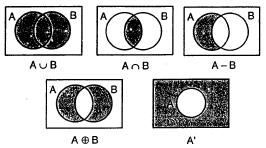
\includegraphics[width=7.5cm,keepaspectratio]{mtran_ima2}}
\caption{Biểu đồ Venn biểu diễn các phép toán tập hợp}
\label{fig:mtran_ima2}
\end{center}
\end{figure}
Đây là một trường hợp, mà chúng ta có thể dùng các logic mệnh đề để chứng minh.
Biểu đồ Venn được sử dụng ở bất kỳ nơi nào trong việc phát triển phần mềm: cùng với đồ thị có hướng, chúng là cơ sở của các ký hiệu trong biểu đồ trạng thái (StateCharts), cái mà là những kỹ thuật chuyên ngành chặt nhất được hỗ trợ bởi kỹ thuật CASE, biểu đồ trạng thái cũng là các ký hiệu điều khiển được dùng cho UML, Ngôn ngữ mô hình hóa toàn cầu (The Universal Modeling Language) của công ty Rational Corp và nhóm quản lý các đối tượng (Object Management Group)
Phép tích đề các của hai tâp tập hợp thì phức tạp hơn; nó phụ thuộc vào các hiệu của các cặp có thứ tự, là những tập hợp có hai phần tử mà trong đó các thứ tự của các phần tử này là rất quan trọng. Chúng ta ký hiệu các cặp có thứ tự và không có thứ tự như sau:

\begin{center}
$\left(a, b\right) = \left(b, a\right) $ nhưng $ \langle a, b \rangle \neq \langle b, a \rangle$
\end{center}

Sự phân biệt này là quan trọng khi tìm hiểu chương 4; như chúng ta đã biết, sự khác nhau căn bản giữa đồ thị thông thường và đồ thị có hướng chính xác là sự khác nhau giữa các cặp không có thự tự và có thứ tự.

\begin{modeling_def}
Tích đề các của hai tập hợp A và B là một tập hợp A \times B = \left\{\left\langle x, y\right\range : x \in A \land  x \in B \right\}.\\
\end{modeling_def}
\\
Biểu đồ Venn không biểu diễn được phép tích đề các, do đó chúng ta sẽ xem một ví dụ đơn giản. Phép tích đề các của các tập hợp A = \left\{1, 2\right\}, B = \left\{a, b\right\} $ là một tập hợp:$

\begin{center}
$A \times B = \left\{\langle 1, a \rangle , \langle 1, b \rangle , \langle 2, a \rangle , \langle 2, b \rangle \right\}$
\end{center}
\newline
Phép tích đề các có một mối liên hệ trực giác với số học. Bản số của một tập hợp A là số các phần tử trong tập hợp A và được ký hiệu là \lvert A \rvert $ (một số tác giả khác gọi lại Card(A)).$  $Cho tập A và B$, \lvert A \times B \rvert = \lvert A \rvert \times \lvert B \rvert. \\

Khi chúng ta nghiên cứu phần kiểm thử chức năng trong chương 5, chúng sẽ sử dụng tích đề các để mô tả các ca kiểm thử cho các chương trình với một vài biến đầu vào. Các thuộc tính bội của một tích đề các có nghĩa là chức năng kiểm thử tạo ra vô số các trường hợp kiểm thử khác.

\subsection {Mối quan hệ giữa các tập hợp}
Chúng ta sử dụng các phép toán tập hợp để xây dựng một số các tập hợp mới từ những tập hợp đã tồn tại. Khi chúng ta làm, chúng ta thường muốn tìm hiểu về một quan hệ giữa các tập hợp mới và các tập hợp cũ (ban đầu) như thế nào. Cho hai tập hợp A và B, chúng ta sẽ định nghĩa ba mối quan hệ tập hợp cơ bản:

\begin{modeling_def}
A là tập con của B, được viết là A \subseteq B, $ khi và chỉ khi $ a \in A \Rightarrow a \in B
$ A là tập con thực sự của B, viết là $ A \subset B, $ khi và chỉ khi $ A \subseteq B \land B - A \neq {\O}\\
$A và B là các tập hợp bằng nhau, viết là A = B$, $ khi và chỉ khi $ A \subseteq B \land B \subseteq A
\end{modeling_def}
\\
\\
Trong tiếng anh hàng ngày, tập hợp A là một tập hợp con của tập hợp B nếu mỗi phần tử của tập hợp A cũng là phần tử của tập B. Để A trở thành một tập con thật sự của B, A phải là một tập con của B và phải có một số phần tử trong B nhưng không phải là phần tử của A. Cuối cùng thì các tập hợp A và B gọi là bằng nhau nếu mỗi tập hợp này là tập con của tập hợp khác.

\subsection {Các cách phân hoạch tập hợp}
Một cách phân hoạch tập hợp là một việc đặc biệt quan trọng cho các kiểm thử. Các phân chia sẽ có một vài tương tự như trong cuộc sống hàng ngày; chung ta có thể dụng sự phận chia để chia tách một vùng của văn phòng lớn thành các văn phòng riêng biệt; chúng ta cũng phải đối mặt với sự phân chia về chính trị khi một quốc gia được chia thành nhiều các đơn vị hành chính (như các thành phố, tỉnh,\dots). Trong cả hai ví dụ này, cần chú ý rằng tính chất của “sự phần chia” là để chia toàn bộ thành các phần nhỏ hơn, cái mà mọi thứ ở trong một vài phần, và không có cái nào bị loại bỏ ra ngoài. Cụ thể là:

\begin{modeling_def}
Cho một tập B và một tập các tập con A1, A2, \dots, An = B, các tập con này là phân hoạch (cách phân chia) của tập B nếu và chỉ nếu A1 \cup A2 \cup \dots \cup An = B $ và $ i \neq j \Rightarrow Ai \cap Aj = \emptyset; i, j =\overline{1, n}.
\end{modeling_def}
\\
\\
Bởi vì một phân hoạch là một tập của các tập con, chúng ta thường gọi là các các tập con riêng biệt như là các phần tử của sự phân hoạch. Hai phần của định nghĩa này là rất quan trọng đối với kiểm thử. Phần thứ nhất đảm bảo rằng mọi phần tử của B là trong một số tập con, trong khi phần thứ hai đảm bảo rằng không có phần tử nào của B thuộc hai tập con.
\begin{figure}[htb]
\setlength\fboxsep{1mm}
\setlength\fboxrule{1pt}
\begin{center}
\fbox{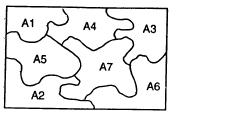
\includegraphics[width=7.5cm,keepaspectratio]{mtran_ima3}}
\caption{Biểu đồ Venn của một phân hoạch}
\label{fig:mtran_ima3}
\end{center}
\end{figure}

Một trò chơi ghép hình là một vị dụ tốt về sự phân hoạch, trong thực tế, các biểu đồ Venn của các phân hoạch được được vẽ giống như các trò chơi ghép hình, như hình \ref{fig:mtran_ima3}.

Sự phân hoạch rất hữu ích cho các testers bởi vì hai thuộc tính trên (định nghĩa) đảm bảo hai yếu tố: sự hoàn chỉnh và không dư thừa. Khi chúng ta nghiên cứu kiểm thử chức năng, chúng ta sẽ nhận thấy rằng những điểm yếu rõ ràng của nó gây ra sự thiếu hụt và sự dư thừa: một số thứ thì không được kiểm thử, trong khi những thứ khác lại được kiểm thử đi kiểm thử lại. Một trong những khó khăn của kiểm thử chức năng tập trung vào việc tìm kiếm một phân hoạch phù hợp. Ví dụ như trong chương trình tam giác (Triangle Program), tập vũ trụ là tập hợp tất cả các bộ ba số nguyên dương. (Chú ý rằng đây thực sự là một tích đề các của tập các số nguyên dương được lặp lại ba lần). Chúng ta có thể phân hoạch tập vũ trụ theo hai cách:
\begin{enumerate}
\item Thành tam giác và phi tam giác
\item Thành tam giác đều, tam giác cân, tam giác không cân, tam giác vuông và phi tam giác
\end{enumerate}
Mới đầu các phân hoạch này dường như là được, nhưng sẽ có một vấn đề với các phân hoạch cuối cùng. Các tập hợp của tam giác cân và tam giác vuông sẽ không bị tách rời (tam giác với các cạnh 3, 4, 5 là một tam giác vuông, đồng thời cũng là tam giác không cân.)

\subsection {Đồng nhất thức tập hợp}
Các phép toán và các mối liên hệ tập hợp, khi được kết hợp với nhau sẽ tạo ra một lớp quan trọng gồm các đồng nhất thức được sử dụng để đơn giản hóa bằng phương pháp đại số các biểu thức tập hợp phức tạp. Các sinh viên toán học thường phải bắt đầu từ tất cả điệu này, chúng ta sẽ chỉ liệt kê và thường xuyên sử dụng chúng như ở hình \ref{fig:mtran_ima4}.
\begin{figure}[htb]
\setlength\fboxsep{1mm}
\setlength\fboxrule{1pt}
\begin{center}
\fbox{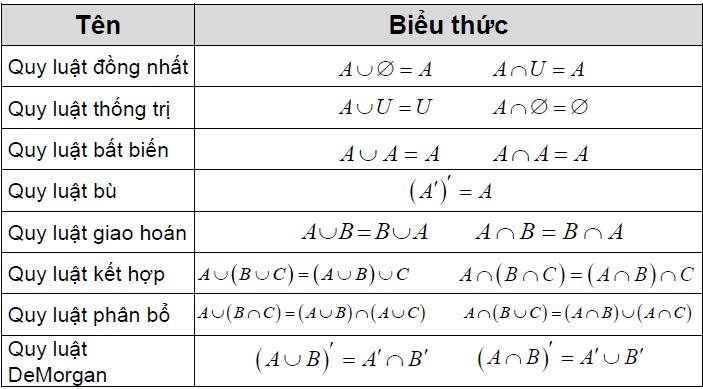
\includegraphics[width=10cm,keepaspectratio]{mtran_ima4}}
\caption{Các đồng nhất thức tập hợp}
\label{fig:mtran_ima4}
\end{center}
\end{figure}

\section{Các hàm}
Các hàm là một khái niệm trọng tâm của phát triển phần mềm và kiểm thử. Ví dụ, mô hình phân tích hàm toàn bộ hoàn toàn sử dụng các khái niệm toán học của một hàm. Chúng ta sẽ làm rõ khái niệm này ở đây bởi vì tất cả kiểm thử hàm (kiểm thử chức năng) dựa trên khái niệm này.

Nói một cách dân dã, một hàm kết hợp các phần tử của các tập hợp. Ví dụ, trong các chương trình Nextdate. Hàm của một ngày đã cho là ngày của ngày tiếp theo, và trong vấn đề tam giác, hàm của ba số nguyên đã cho là loại tam giác được tạo bởi các cạnh với các độ dài đã cho. Trong vấn đề tiền hoa hồng, hoa hồng của người bán là một hàm của việc bán hàng, nó lần lượt là một hàm của số lượng khóa, lượng cổ phần và số thùng được bán. Các hàm trong hệ thống ATM phức tạp hơn nhiều, không ngạc nhiên rằng, điều này sẽ làm tăng sự phức tạp cho quá trình kiểm thử. 
Bất cứ một chương trình nào có thể được coi là một hàm, các đầu vào là các miền (domain) và các sản phẩm là một loạt các hàm. 

\begin{modeling_def}
Cho 2 tập hợp A và B , một hàm f là một tập con của A \times B.\\
$Cho $ a_{i}, a_{j} \in A, b_{i}, b_{j} \in B, $ và $ f\left(a_{i}\right) = b_{i}, f\left(a_{j}\right) = b_{j}, b_{i} \neq b_{j} \Rightarrow a_{i} \neq a_{j}.
\end{modeling_def}
\\
\\
Các định nghĩa chính thức như trên khá ngắn gọn, do vậy chúng ta hãy xem xét kỹ hơn. Các đầu vào đối với hàm f là các phần tử của tập hợp A, và các đầu ra của f là các phần tử của B. Những định nghĩa chỉ ra rằng hàm được xem xét kỹ lưỡng ở chỗ một phần tử trong tập hợp A chưa bao giờ kết hợp với hơn một phần tử của B. Nếu điều này có thể xảy ra, chúng ta đã từng kiểm thử một hàm như thế nào?. Đây là một ví dụ không tất định. 

\subsection{Miền và phạm vi}
Trong khái niệm vừa ra, tập hợp A là một miền của hàm f, và tập hợp B là phạm vi. Bởi vì đầu vào và đầu ra có một thứ tự “tự nhiên”, thật là đơn giản để nói rằng một hàm thực sự là một tập hợp gồm các cặp có thứ tự cái mà phần tử đầu tiên là từ miền và phần tử thứ hai là từ phạm vi. Đây là hai ký hiệu cho hàm:  $f \subseteq A \times B$. \\
Chúng ta không đặt bất kỳ hạn chế nào trên các tập A và B trong định nghĩa này. Chúng ta có thể có 
A = B, vả cả A hoặc B có thể là một tích đề các của các tập hợp khác.

\subsection{Các loại hàm}
Các hàm sẽ được mô tả kỹ lưỡng hơn bởi phép ánh xạ. Trong định nghĩa dưới đây, chúng ta bắt đầu với một f : A \to B, $ và chúng ta định nghĩa một tập hợp:$\\
$f\left(A\right) = \left\{b_{i} \in B : b_{i} =  f\left(a_{i}\right) $ với một vài $ a_{i} \in A \right\}.$\\

Tập hợp này đôi khi được gọi là hình ảnh của A dưới hàm f.

\begin{modeling_def}
f là một hàm từ A đến B khi và chỉ khi f\left(A\right) = B.\\
$f là một hàm từ A vào B khi và chỉ khi $ f\left(A\right) \subset B $(chú ý các tập con thích hợp ở đây).$\\
$f là một hàm ánh xạ một một từ A đến B khi và chỉ khi, cho mọi:$  \\
$a_{i}, a_{j} \in A, a_{i} \neq a_{j} \Rightarrow f\left(a_{i}\right) \neq f\left(a_{j}\right).$\\
f là một hàm ánh xạ từ nhiều đến một từ A đến B khi và chỉ khi, tồn tại a_{i}, a_{j} \in A, a_{i} \neq a_{j} $ mà $ f\left(a_{i}\right) = f\left(a_{j}\right).
\end{modeling_def}
\\
\\
Trở lại tiếng Anh thông dụng, nếu f là một hàm từ A đến (onto) B, chúng ta biết rằng mỗi phần tử của tập B sẽ được kết hợ với vài 1 số phần tử của A. Nếu hàm từ A vào (into) B, chúng ta biếts rằng sẽ có ít nhất một phần tử của B mà không được kết hợp với một phần tử của A. Các hàm ánh xạ một-một đàm bảo một dạng đơn nhất: Các phần tử domain riêng biệt sẽ chưa bao giờ được ánh xạ tới các phần tử trong cùng một dãy. Nếu một hàm không phải là đơn ánh (ánh xạ một một), nó sẽ là ánh xạ từ nhiều đến một (many-to-one), đó là nhiều hơn một phần tử domain có thể được ánh xạ đến phần tử trong cùng một dãy. Trong những thuật ngữ này, các yêu cầu về “đối xử tốt” sẽ ngăn cản các hàm trở thành ánh xạ một đến nhiều (one-to-many). Các tester quên với các dữ liệu có tính chất liên quan sẽ nhận ra rằng tất cả các khả năng (Một đến một, một đến nhiều, nhiều đến một, và nhiều đến nhiều) được cho phép cho các mối quan hệ. 
Trở lại với các ví dụ kiểm thử của chúng ta, giả sử chúng ta lấy A, B, C là các tập hợp các ngày trong chương trình NextDate, nơi mà :\\
\newline
A = \left\{date : 1 \; January \; 1812 \leq date \leq 31 \; December \; 2012 \right\}\\
B = \left\{date : 2 \; January \; 1812 \leq date \leq 1 \; January \; 2013 \right\}\\
C =  A \cup B\\


Bây giờ, NextDate : $ A \to B$  là một ánh xạ một-một, lên hàm( onto function), và NextDate: $A \to C$  là một ánh xạ một-một , vào trong hàm (into function). Ý nghĩa của NextDate không là nhiều tới một, nhưng rất dễ thấy các vấn đề ở hình tam giác có thể là nhiều tới một. Khi một hàm là một tới một và đến (onto), như NextDate $ A \to B $ ở trước, mỗi phần tử của miền tương ứng với đúng một phần tử của của dãy (range); ngược lại, mỗi phần tử của dãy tương ứng với đúng một phần tử của miền. Khi điều này xảy ra. Nó luôn luôn có thể tìm thấy một hàm ngược (có thể nhìn thấy vấn đề YesterDate trong chương 2) đó là một tới một từ dãy trở về miền.
Tất cả điều này là quan trọng để kiểm thử. Định nghĩa vào (into) khác biệt với đến (onto) có ý nghĩa cho tên miền và phạm vi kiểm tra dựa trên kiêm thử chức năng, và các hàm một tới một được yêu cầu kiểm thử nhiều hơn so với các hàm nhiều tới một.

\subsection {Hợp thành hàm}
Giả sử chúng ta có các tập hợp và các hàm như vậy sau:\\
$f : A \to B, g : B \to C, h : C \to D$\\
Khi điều này xảy ra, chúng ta có tạo ra các hàm. Để làm điều này, chúng ta hãy liên hệ đến các phần tử của domain và phạm vi các tập hợp a $ \in A, b \in B, c \in C, d \in D $, và giả sử rằng $ f\left(a\right) = b, f\left(b\right) = c, f\left(c\right) = d$ . Bây giờ sự hợp thành của các hàm g và f  là: \\
$h \circ g \circ f\left(a\right) = h\left(g\left(f\left(a\right)\right)\right) = h\left(g\left(b\right)\right) = h\left(c\right) = d.$\\
\newline
Hàm hợp thành là một ứng dụng rất phổ biến trong phát triển phần mềm; nó được thừa hưởng trong quá trình định nghĩa thủ tục (procedures) và các thủ tục con (subroutines). Chúng ta có một ví dụ về vấn đề này trong chương trình tiền hoa hồng, trong đó:\\
f_{1}\left(locks, stocks, barels\right) = sales\\
f_{2} \left(sales\right) = commission\\

Hàng loạt các hàm được tạo ra có thể gây khó khăn cho testers, đặc biệt khi phạm vi của một hàm là một tập con thích hợp của domain của hàm “tiếp theo” trong hàng loạt các hàm. Hình \ref{fig:mtran_ima5} biểu diễn nó có thể xảy ra như thế nào trong một chương trình được định nghĩa bởi biểu đồ luồng dữ liệu.
Trong causal flow (luồng nhân quả), g.f(a) (cái mà chúng ta biết kết quả sẽ là g(b), g(b) lại tạo ra c) là một quá trình khá giống như assemblyline-like. Trong luồng không nhân quả (nocausal flow), khả năng nhiều hơn một tài nguyên của các giá trị b cho kho dữ liệu B sẽ gây ra hai vấn đề cho testers. Nhiều nguồn của các giá trị b có thể gây lên những vấn đề khả năng tương thích về domain/range(phạm vi); và thậm chí nếu điều này không phải là một vấn đề, có thể sẽ có bất thường thời gian đối với các giá trị của b. 

Một trường hợp đặc biệt của hợp thành có thể được sử dụng, giúp kiểm tra một cách tò mò (curious). Nhớ lại chúng ta đã thảo luận làm thế nào đơn ánh (one-to-one) vào các hàm có một hàm ngược (hàm nghịch đảo). Nó chỉ ra rằng hàm ngược này là duy nhất và được đảm bảo tồn tại. 

\begin{figure} [htb]
\setlength\fboxsep{1mm}
\setlength\fboxrule{1pt}
\begin{center}
\fbox{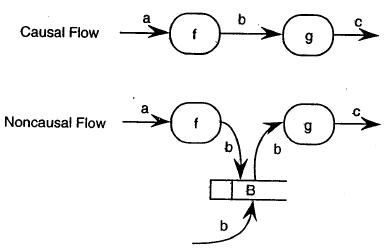
\includegraphics[width=7.5cm,keepaspectratio]{mtran_ima5}}
\caption{Luồng nhân quả và không nhân quả trong biểu đồ luồng dữ liệu}
\label{fig:mtran_ima5}
\end{center}
\end{figure}

Nếu f là một hàm đơn ánh từ A vào B, chúng ta biểu thị hàm ngược bởi  $f^{-1}$. Nó chỉ ra rằng $ a \in A $ và $b \in B, f^{-1}. f\left(a\right) = a $ và $ f^{-1}$ . $f\left(b\right) = b. $ Các chương trình NextDate và YesterDate được biết đến như là một ánh xạ ngược. Có một cách giúp kiểm thử là, đối với một hàm nhất định, ánh xạ ngược của nó như là một “kiểm tra chéo”, và điều này thường có thể tiến hành việc xác định các trường hợp thử nghiệm chức năng.

\section{Các quan hệ}
Hàm là trường hợp đặc biệt của quan hệ: cả hai đều là tập con của một số tích Đề
các, nhưng trong trường hợp hàm, chúng ta có yêu cầu "hoạt động tốt" mà nói rằng
một phần tử miền không thể được kết hợp với nhiều hơn một phần tử phạm vi. Điều
này sinh ra trong cách sử dụng hàng ngày: khi chúng ta nói cái gì đó "là một
hàm" của một cái khác, mục đích là đưa ra một quan hệ tất định. Không phải tất
cả các mối quan hệ là hàm. Xem xét ánh xạ giữa một tập hợp các bệnh nhân và một
tập các bác sĩ. Một bệnh nhân có thể được điều trị bởi một vài bác sĩ, và một
bác sĩ có thể điều trị một vài bệnh nhân, một ánh xạ nhiều-nhiều. Việc xác định
quan hệ giữa các tập (các lớp đối tượng), các thành phần trong một tập cũng như
các tính chất của quan hệ, giúp nâng cao hiệu quả kiểm thử, sinh testcase, mô
hình hóa dữ liệu...

\subsection{Quan hệ giữa các tập}
Hãy bắt đầu với một định nghĩa.
\begin{modeling_def}
Cho hai tập A và B, một quan hệ R là một tập con của tích Đề các $ A \times B $.
\end{modeling_def}

Hai ký hiệu phổ biến; khi chúng ta muốn nói về mối quan hệ toàn bộ, chúng ta thường viết $ R \subseteq A \times B $ cho các phần tử cụ thể $ a_{i} \in A, b_{i} \in B $, chúng ta viết $ a_{i} R b_{i} $. Hầu hết các văn bản toán học bỏ qua xử lý của các quan hệ; chúng ta quan tâm đến chúng vì chúng cần thiết cho cả mô hình hóa dữ liệu và phân tích hướng đối tượng.\\
Tiếp theo, chúng ta phải giải thích thuật ngữ – lực lượng. Hãy nhớ lại rằng vì nó áp dụng cho các tập, lực lượng là số phần tử trong một tập. Vì một quan hệ cũng là một tập, chúng ta có thể hy vọng rằng lực lượng của một quan hệ liên quan đến bao nhiêu cặp đã cho nằm trong tập $ R \subseteq A \times B $. Thật không may, điều này không đúng.

\begin{modeling_def}
Cho hai tập A và B, một quan hệ $ R \subseteq A \times B $, lực lượng của quan hệ R là:\\
Một – một khi và chỉ khi R là một hàm một – một từ A đến B,\\
Nhiều – một khi và chỉ khi R là một hàm nhiều – một từ A đến B,\\
Một – nhiều khi và chỉ khi có ít nhất một phần tử $ a \in A $ ở trong hai cặp đã cho trong R, mà $ (a, b_{i}) \in R $ và $ (a, b_{j}) \in R $,\\
Nhiều – nhiều khi và chỉ khi có ít nhất một phần tử $ a \in A $ trong hai cặp đã cho trong R, mà $ (a, b_{i}) \in R $ và $ (a, b_{j}) \in R $; và có ít nhất một phần tử $ b \in B $ trong hai cặp đã cho trong R, mà $ (a_{i}, b) \in R $ và $ (a_{j}, b) \in R $.
\end{modeling_def}

Sự khác biệt giữa các hàm với phạm vi của nó tương tự như các quan hệ - khái niệm về sự tham gia.
\begin{modeling_def}
Cho hai tập A và B, một quan hệ $ R \subseteq A \times B $, sự tham gia của quan hệ R là:\\
\begin{itemize}
\item Toàn bộ khi và chỉ khi mọi phần tử của A có trong một số cặp đã cho trong R,
\item Từng phần khi và chỉ khi một số phần tử của A không có trong một số cặp đã cho trong R,
\item Onto khi và chỉ khi mọi phần tử của B có trong một số cặp đã cho trong R,
\item Into khi và chỉ khi một số phần tử của B không có trong một số cặp đã cho trong R.
\end{itemize}
\end{modeling_def}

Diễn đạt một cách đơn giản, một quan hệ là toàn bộ nếu nó áp dụng cho mọi phần tử của A, và từng phần nếu không áp dụng cho mọi thành phần. Thuật ngữ khác cho sự phân biệt này là sự tham gia bắt buộc và tùy chọn. Tương tự như vậy, một quan hệ onto nếu nó áp dụng cho mọi phần tử của B, và into nếu không. Sự tương tương giữa toàn bộ/từng phần và onto/into là kì lạ, và xứng đáng được đề cập đặc biệt ở đây. Từ quan điểm của lý thuyết cơ sở dữ liệu quan hệ, thì không có lý luận gì cho điều này; trong thực tế, có một lý luận thuyết phục để tránh sự phân biệt này. Mô hình hóa dữ liệu chủ yếu là khai báo, trong khi quá trình mô hình hóa chủ yếu là bắt buộc. Các tập tương đương của các thuật ngữ tạo ra một hướng trên các quan hệ, trong khi thực tế không cần sụ định hướng này. Một phần của điều này là từ thực tế rằng các tích Đề các bao gồm các cặp đã cho, rõ ràng có một phần tử đầu và thứ hai.

Cho đến đây, chúng ta chỉ xem xét các quan hệ giữa hai tập. Việc mở rộng các quan hệ với ba hay nhiều tập là phức tạp hơn tích việc tính tích Đề các một cách đơn giản. Ví dụ, giả sử chúng ta có có ba tập A, B, và C, và một quan hệ $ R \subseteq A \times B \times C $. Chúng ta muốn quan hệ được chặt chẽ giữa ba phần tử, hay giữa một phần tử và một cặp đã cho (sẽ có ba khả năng ở đây)? Hướng suy luận này cũng cần phải áp dụng cho các định nghĩa của lực lượng và sự tham gia. Nó là đơn giản cho sự tham gia, nhưng lực lượng là một thuộc tính nhị phân. (Ví dụ, giả sử quan hệ là một – một từ A sang B, và nhiều – một từ A đến C). Chúng ta thảo luận về quan hệ ba bên ở Chương 1, khi chúng ta kiểm tra các mối quan hệ giữa các hành vi chương trình được đặc tả, được triển khai, và kiểm thử. Chúng ta muốn có một dạng tập hợp giữa các trường hợp kiểm thử và các cặp đặc tả - cài đặt; chúng ta sẽ xem xét lại điều này khi nghiên cứu về kiểm thử chức năng và cấu trúc.

Kiểm thử viên cần phải được liên hệ với các định nghĩa về quan hệ bởi vì họ liên quan một cách trực tiếp đến các thuộc tính phần mềm được kiểm thử. Ví dụ, sự phân biệt onto/into liên quan trực tiếp đến những gì chúng ta sẽ yêu cầu dữ liệu ra dựa trên kiểm thử chức năng. Sự phân biệt bắt buộc – tuỳ chọn là bản chất của việc xử lý ngoại lệ, cũng có ý nghĩa đối với kiểm thử viên.

\subsection{Quan hệ trong một tập đơn}
Có hai quan hệ toán học quan trọng được định nghĩa trong một tập đơn là: quan hệ thứ tự và quan hệ tương đương. Cả hai được định nghĩa vớ các thuộc tính cụ thể của quan hệ.

Đặt A là một tập, và $ R \subseteq A \times A $ một quan hệ được định nghĩa trên A, với $ <a,a>, <a,b>, <b,a>, <b,c>, và <a,c> \in R $. Có bốn thuộc tính đặc biệt của quan hệ:

\begin{modeling_def}
Một quan hệ $ R \subseteq A \times A $:\\
\begin{itemize}
\item Phản xạ khi và chỉ khi với mọi $ a \in A, <a,a> \in R $,
\item Đối xứng khi và chỉ khi $ <a,b> \in R \Rightarrow <b,a> \in R $,
\item Phản đối xứng $ <a,b>, <b,a> \in R \Rightarrow a=b $,
\item Bắc cầu khi và chỉ khi $ <a,b>, <b,c> \in R \Rightarrow <a,c> \in R $.
\end{itemize}
\end{modeling_def}

Các mối quan hệ gia đình là những ví dụ hay về các thuộc tính này. Bạn có thể
suy nghĩ về các mối quan hệ sau, và quyết định thuộc tính nào được áp dụng: anh trai của, anh chị em ruột của, tổ tiên của. Bây giờ, chúng ta có thể định nghĩa hai quan hệ quan trọng.

\begin{modeling_def}
Một quan hệ $ R \subseteq A \times A $ là một quan hệ thứ tự nếu R có tính phản xạ, phản đối xứng, và bắc cầu.
\end{modeling_def}

Quan hệ thứ tự có một chiều định hướng; một số quan hệ thứ tự phổ biến là già hơn, $ \Rightarrow $ hay $ \geq $, và tổ tiên của. (các phần phản xạ thường yêu cầu một vài biến đổi – chúng ta không nói trẻ hơn và không phải là con cháu của). Quan hệ thứ tự xuất hiện phổ biến trong phần mềm: các kỹ thuật truy cập dữ liệu, mã băm, cấu trúc cây, và mảng là tất cả các trường hợp mà quan hệ thứ tự được sử dụng.

Tập lực lượng của của một tập là tập của tất cả các tập con của tập đó. Tập lưc lượng của tập A được kí hiệu là P(A). Quan hệ tập con $ \subseteq $ là một quan hệ thứ tự trên P(A), vì nó có tính phản xạ (tập nào cũng là tập con của chính nó), nó có tính phản đối xứng (định nghĩa tập bằng nhau), và nó có tính bắc cầu.

\begin{modeling_def}
Một quan hệ $ R \subseteq A \times A $ là một quan hệ tương đương nếu R có tính phản xạ, đối xứng, và bắc cầu.
\end{modeling_def}

Toán học có đầy đủ quan hệ tương đương: đẳng thức và đồng dư thức là hai ví dụ. Có một kết nối quan trọng giữa quan hệ tương đương và sự phân chia của một tập. Giả sử chúng ta có các phần $ A_{1}, A_{2}, …, A_{n} $ của một tập B, và chúng ta nói rằng hai phần tử $b_{1}$ và $b_{2}$ của B có quan hệ (ví dụ $b_{1}$ R $b_{2}$) nếu $b_{1}$ và $b_{2}$ ở trong cùng một phân vùng. Quan hệ này có tính phản xạ (phần tử nào cũng ở trong chính phân vùng của nó), có tính đối xứng (nếu $b_{1}$ và $b_{2}$ ở trong một phân vùng, thì $b_{2}$ và $b_{1}$ cũng thế), và có tính bắc cầu (nếu $b_{1}$ và $b_{2}$ ở trong cùng một tập, và nếu $b_{2}$ và $b_{3}$ ở trong cùng một tập, thì $b_{1}$ và $b_{3}$ ở trong cùng một tập). Quan hệ mà được định nghĩa từ phân vùng được gọi là quan hệ tương đương được gây ra bởi phân vùng. Quá trình ngược lại hoạt động tương tự. Nếu chúng ta bắt đầu với một quan hệ tương đương được định nghĩa trên một tập, chúng ta có thể định nghĩa một tập con theo các phần tử mà có liên quan với nhau. Đây là một phân vùng và được gọi là phân vùng được tạo ra bởi quan hệ tương đương. Các tập ở trong phân vùng này được biết như là các lớp tương đương. Kết quả cuối cùng là các phân vùng và các quan hệ tương đương đó có thể hoán đổi và điều này trở thành một khái niệm mạnh mẽ cho các kiểm thử viên. Hãy nhớ lại rằng hai thuộc tính của một phân vùng là khái niện đầy đủ và không dư thừa. Khi được dịch sang các tình huống kiểm thử, những khái niệm này cho phép các kiểm thử viên tạo ra các trình bày tuyệt đối về quy mô mà các thành phần phần mềm đã được kiểm thử. Ngoài ra, hiệu quả từ việc kiểm thử chỉ là một phần tử của một lớp tương đương, và giả sử rằng các thành phần còn lại sẽ hoạt động tương tự.

\section{Logic mệnh đề}
Chúng ta đã từng sử dụng ký hiệu logic mệnh đề; nếu bạn đang lúng túng bởi này sử dụng trước khi định nghĩa, bạn không phải là người duy nhất. Lý thuyết tập hợp và logic mệnh đề có mối quan hệ con gà và quả trứng - thật khó để quyết định cái gì cần được thảo luận đầu tiên. Một mệnh đề là một câu hoặc là đúng hoặc sai, và chúng ta gọi những giá trị này là giá trị chân lý của mệnh đề. Hơn nữa, các mệnh đề là rõ ràng: một mệnh đề được đưa ra, nó luôn cho biết đó là đúng hay sai. Câu "Toán học khó" sẽ không đủ điều kiện là một mệnh đề vì nó mơ hồ. Chúng ta thường biểu thị các mệnh đề với các chữ cái thường p, q và r. Mệnh đề logic có các phép toán, biểu thức, và định danh mà tương tự như lý thuyết tập hợp (trong thực tế chúng là đẳng cấu).

\subsection{Toán tử logic}
Toán tử logic (còn được biết như là các phần tử kết nối hay phép toán logic) được định nghĩa trong thuật ngử của tác động của chúng trên giá trị chân lý của mệnh đề mà chúng được áp dụng. Điều này là dễ dàng, vì chỉ có hai giá trị: T (đúng) và F (sai). Toán tử số học cũng có thể được định nghĩa theo cách này, (trong thực thế, đó là cách chúng được dạy cho trẻ con), nhưng các bảng trở nên rất lớn. Ba toán tử logic cơ bản là và ($\wedge$), hoặc ($\vee$) và không ($\urcorner$); những toán tử này đôi khi được gọi là hội, tuyển, và phủ định. Phủ định là toán hạng logic đơn nguyên (một toán hạng); những toán tử khác là nhị nguyên.

\begin{table}
\centering
\caption{Bảng chân lý của các toán tử cơ bản}
\begin{tabular}{|c|c|c|c|c|l|} 
\hline p&q&p $\wedge$ q&p $\vee$ q&$\urcorner$p\\ 
\hline T&T&T&T&F\\ 
\hline T&F&F&T&F\\ 
\hline F&T&F&T&T\\ 
\hline F&F&F&F&T\\
\hline\end{tabular}
\end{table}

Tuyển và hội phổ biến trong cuộc sống hằng ngày: một hội là đúng chỉ khi tất cả các thành phần là đúng, và một tuyển là đúng nếu ít nhất một thành phần là đúng. Phủ định cũng hoạt động như chúng ta mong đợi. Có hai kết nối phổ biến loại trừ tuyển ($\oplus$) và nếu – thì ($\rightarrow$); chúng được định nghĩa như sau:

\begin{table}
\centering
\caption{Bảng chân lý của phép loại trừ tuyển và nếu - thì}
\begin{tabular}{|c|c|c|c|l|} 
\hline p&q&p $\oplus$ q&p $\rightarrow$ q\\ 
\hline T&T&F&T\\ 
\hline T&F&T&F\\ 
\hline F&T&T&T\\ 
\hline F&F&F&T\\
\hline\end{tabular}
\end{table}

Một phép loại trừ tuyển là đúng chỉ khi một trong các mệnh đề là đúng, trong khi một tuyển là đúng nếu cả hai mệnh để là đúng. Kết nối nếu – thì thường gây ra khó khăn nhất. Vì các toán tử khác đều chuyển sang ngôn ngữ tự nhiên, nên chúng ta có mong muốn tương tự với nếu – thì. Câu trả lời nhanh là toán tử nếu – thì quan hệ chặt chẽ với quá trình suy luận: trong một tam đoạn luận hợp lệ, chúng ta có thể nói “nếu cơ sở, thì kết luận” và nếu – thì là một phép lặp thừa.

\subsection{Biểu thức logic}
Chúng ta sử dụng các toán tử logic để xây dựng các biểu thức logic một cách chính xác như chúng ta sử dụng các toán tử số học để xây dựng các biểu thức đại số. Chúng ta có thể xác định thứ tự mà các toán tử được áp dụng với các quy ước thông thường theo các dấu ngoặc đơn, hoặc chúng ta có thể sử dụng thứ tự ưu tiên (phủ định đâu tiên, sau đó là hội và cuối cùng là tuyển). Cho một biểu thức logic, chúng ta có thể luôn luôn tìm bảng chân lý của nó bằng cách xây dựng theo thứ tự được xác định bởi các dấu ngoặc đơn. Ví dụ, biểu thức $\urcorner$((p$\rightarrow$q)$\wedge$(q$\rightarrow$p)) có bẳng chân lý sau:

\begin{table}
\centering
\caption{Bảng chân lý của biểu thức
$\urcorner$((p$\rightarrow$q)$\wedge$((q$\rightarrow$p))}
\begin{tabular}{|c|c|c|c|l|} 
\hline $\rightarrow$q&$\rightarrow$p&(p$\rightarrow$q)$\wedge$((q$\rightarrow$p)&$\urcorner$((p$\rightarrow$q)$\wedge$((q$\rightarrow$p))\\ 
\hline F&F&T&F\\ 
\hline F&T&F&T\\ 
\hline T&F&F&T\\ 
\hline T&T&T&F\\
\hline\end{tabular}
\end{table}

\subsection{Tương đương}
Các khái niệm về đẳng thức số học và các tập giống nhau tương tự trong mệnh đề logic. Chú ý rằng biểu thức $\urcorner$((p$\rightarrow$q)$\wedge$(q$\rightarrow$p)) và p$\oplus$q có bẳng chân lý giống nhau. Điều này có nghĩa là, không quan tâm giá trị chân lý được đưa ra bởi các mệnh đề p và q là gì, các biểu thức này sẽ luôn có cùng giá trị chân lý. Có một vài cách để định nghĩa thuộc tính này, chúng ta cách sử dụng đơn giản nhất.

\begin{modeling_def}
Hai mệnh đề p và q là tương đương logic (kí hiệu là p $\Leftrightarrow$ q) khi chỉ khi bảng giá trị chân lý của chúng giồn nhau.
\end{modeling_def}

Tiện thể, chữ viết tắt “iff” chúng tả sử dụng cho “khi và chỉ khi” đôi khi được gọi là hai điều kiện, do đó mệnh đề p iff q là (p$\rightarrow$q)$\wedge$(q$\rightarrow$p), được kí hiệu là p$\Leftrightarrow$q.

\begin{modeling_def}
Một mệnh đề luôn đúng là một phép lặp thừa; một mệnh đề luôn sai là một phủ định.
\end{modeling_def}

Để một là phép lặp thừa hoặc phủ định, một mệnh đề phải chứa ít nhất một liên kết và hai hoặc nhiều nhiều mệnh đề nguyên thủy. Chúng ta đôi khi biểu thị một phép lặp thừa như một mênh đề T, và một phủ định như một mệnh đề F. Chúng ta có thể đặt ra một vài luật mà điều kiển sự tương đương chúng ta có cho các tập.

\begin{table}
\centering
\caption{Các luật tương đương}
\begin{tabular}{|c|c|l|} 
\hline Luật&Biểu thức\\
\hline Đồng nhất&p $\wedge$ T $\Leftrightarrow$ p, p $\vee$ F $\Leftrightarrow$ p\\ 
\hline Ưu thế&p $\vee$ T $\Leftrightarrow$ T, p $\wedge$ F $\Leftrightarrow$ F\\ 
\hline Lũy đẳng&p $\wedge$ p $\Leftrightarrow$ p, p $\vee$ p $\Leftrightarrow$ p\\ 
\hline Bù&$\urcorner$($\urcorner$p) $\Leftrightarrow$ p\\
\hline Giao hoán&p $\wedge$ q $\Leftrightarrow$ q $\wedge$ p, p $\vee$ q $\Leftrightarrow$ q $\vee$ p\\
\hline Kết hợp&p $\wedge$ (q $\wedge$ r) $\Leftrightarrow$ (p $\wedge$ q) $\wedge$ r, p $\vee$ (q $\vee$ r) $\Leftrightarrow$ (p $\vee$ q) $\vee$ r\\
\hline Phân phối&p $\wedge$(q $\vee$ r) $\Leftrightarrow$ (p $\wedge$ q) $\vee$ (p $\wedge$ r), p $\vee$ (q $\wedge$ r) $\Leftrightarrow$ (p $\vee$ q) $\wedge$ (p $\vee$ r)\\
\hline De Morgan&$\urcorner$(p $\wedge$ q) $\Leftrightarrow$ $\urcorner$p $\vee$ $\urcorner$q, $\urcorner$(p $\vee$ q) $\Leftrightarrow$ $\urcorner$p $\wedge$ $\urcorner$q \\
\hline\end{tabular}
\end{table}

Áp dụng các luật tương đương cho phép biến đổi rút gọn các điều kiện ràng
buộc, qua đó tăng hiệu quả kiểm thử mà không phải đi qua những trường hợp có thể
không thể xảy ra hoặc có xảy ra nhưng không ảnh hưởng đến kết quả cần kiểm thử.
\section{Lý thuyết xác suất}
Chúng ta sẽ có hai lần sử dụng lý thuyết xác suất trong nghiên cứu của chúng ta về kiểm thử phần mềm: xác suất một đường thực thi các lệnh cụ thể, và tổng quát hóa cái này cho khái niệm công nghiệp được gọi là “thông tin hoạt động” (xem chương 14). Vì điều này hạn chế sử dụng, nên chúng ta sẽ chỉ quan tâm đến các cơ sở kiến thức ở đây.

Như với cả lý thuyết tập hợp và mệnh đề logic, chúng ta bắt đầu với một khái niệm nguyên thủy – xác suất của một sự kiện. Đây là định nghĩa được cung cấp bởi một sách giáo khoa hiện tại [Rosen 91]: “Xác suất của một sự kiện E, là một tập con của một không gian mẫu hữu hạn S của các suy luận logic có khả, là p(E) = $\mid$E$\mid$ / $\mid$S$\mid$”. Định nghĩa này xoay quanh ý tưởng kinh nghiệm mà kết quả là một suy luận logic, không gian mẫu là tập tất cả các suy luận có thể, và một sự kiện là một tập cọn của các suy luận. Định nghĩa này bị luẩn quẩn: các suy luận tương đương là gì? Chúng ta giả sử những cái này có xác suất bằng nhau, nhưng sau đó xác suất được định nghĩa ở trong chính nó.

Nhà toán học người Pháp Laplace đã có một định nghĩa xác suất hai thế kỉ trước. Để diễn giải nó, xác suất mà một cái gì đó xảy ra la số các thuận tiện nó có thể xảy ra chia cho tổng số cách (thuận tiện và không). Định nghĩa của Laplace làm việc tốt khi chúng ta quan tâm đến việc vẽ các hòn bi được tô màu ngoài một cái túy, nhưng không mở rộng tốt cho các trường hợp mà khó liệt kê các khả năng khác nhau.

Chúng ta sẽ sử dụng khả năng của chúng ta trong lý thuyết tập hợp và mệnh đề logic để đi dến một công thức gắn kết hơn. Là một kiểm thử viên, chúng ta sẽ quan tâm đến những thứ xảy ra; chúng ta sẽ gọi những sự kiện này, và nói rằng tập các sự kiện là tập vũ trụ. Tiếp theo, chúng ta sẽ đưa ra các mệnh đề về sự kiện, như mệnh đề liên quan đến các phần tử trong tập vũ trụ. Bây giờ, với một số tập hợp U và một số mệnh đề p về các phần tử của U, chúng ta có một định nghĩa:

\begin{modeling_def}
Tập chân lý T của một mệnh đề p, được viết là T(p), là tập của tất cả các thành phần ở trong tập hợp U với p là đúng.
\end{modeling_def}

Vì các mệnh đề hoặc là đúng hoặc là sai, một mệnh đề p chia tập vũ trụ ra thành 2 tập, T(p) và (T(p))', với T(p) $\cup$ (T(p))' = U. Chú ý rằng (T(p))' giống với T($\urcorner$p). Các tập chân lý tạo ra một ánh xạ rõ rang giữa lý thuyết tập hợp, logic mệnh đề, và lý thuyết xác suất.

\begin{modeling_def}
Xác suất mà một mệnh đề p là đúng, kí hiệu là Pr(p), là $\mid$T(p)$\mid$ / $\mid$U$\mid$.
\end{modeling_def}

Với định nghĩa này, “số lượng các cách thuận tiện” của Laplace trở nên lực lượng của tập chân lý T(p), và tổng số cách trở thành lực lượng của tập vũ trụ. Điều này tạo ra nhiều hơn một liên kết: vì bảng chân lý của một phép lặp thừa là tập vũ trụ, và tập chân lý của một phủ định là tập rỗng, xác suất của $\oslash$ và U là 0 và 1.

Vấn để NextDate là một ví dụ mã nguồn hay. Hãy xem xét biến tháng, và mệnh đề 
\begin{center}
p(m): m là một tháng có 30 ngày
\end{center}

Tập vũ trụ là tập U = (Jan, Feb, …, Dec), và tập chân lý của p(m) là tập
\begin{center}
T(p(m)) = {Apr, June, Sept, Nov}
\end{center}

Bây giờ, xác suất mà một tháng là tháng có 30 ngày là 
\begin{center}
Pr(P(m)) = $\mid$T(p(m))$\mid$ / $\mid$U$\mid$ = 4 / 12
\end{center}

Có một chút không khéo trong vai trò của tập vũ trụ; đây là một phần của kỹ thuật sử dụng lý thuyết xác suất trong kiểm thử - việc chọn đúng tập hợp. Giả sử chúng ta muốn biết xác suất của một tháng là tháng 2. Câu trả lời là 1/12. Bây giờ, giả sử chúng ta muốn xác suất của một tháng có chính sác 29 ngày. Chúng ta cần một tập hợp gồm cả năm nhuận và năm không nhuận. Chúng ta có thể sử dụng đồng dư thức số học, và chọn một tập gồm các tháng trong một khoảng 4 năm liến tiếp, như 1991, 1992, 1993, và 1994. Tập này sẽ chứa 48 tháng, và xác suất của một tháng có 29 ngày là 1/48. Một khẳ năng khác là sử dụng toàn bộ khoảng hai thế của chương trình NextDate, trong đó, năm 2000 không phải là năm nhuận. Điều này sẽ làm giảm xác suất của một tháng có 29 ngày. Kết luận, việc tìm tập vũ trụ là quan trọng. Kết luận lớn hơn: nó thậm chí quan trọng hơn để tránh việc chuyển tập hợp.

Dưới đây là một số cơ sở lập luận về xác suất mà chúng ta sẽ sử dụng mà không cần chứng minh. Chúng liên quan đến tập hợp, mệnh đề p và q, với tập chân lý T(p) và T(q).
\begin{itemize}
\item Pr($\urcorner$p) = 1 - Pr(p)
\item Pr(p $\wedge$ q) = Pr(p) $\wedge$ Pr(q)
\item Pr(p $\vee$ q) = Pr(p) + Pr(q) - Pr(p $\wedge$ q)
\end{itemize}

Những cơ sở lập luận này, cùng với bảng của lý thuyết tập hợp và đồng nhất thức
mệnh đề, cung cấp một khả năng đại số để biến đổi các biểu thức xác suất. Nhằm
cải thiện quá trình sinh testcase, kiểm thử các biên, hoặc có thể chấp nhận một
trường hợp lỗi nào đó nếu như xác suất xảy ra rất thấp ở một mức cho phép của
yêu cầu phần mềm.

\section{Vị thế của toán rời rạc trong các kỹ thuật kiểm thử}
\begin{figure}
\setlength\fboxsep{1mm}
\setlength\fboxrule{1pt}
\begin{center}
\fbox{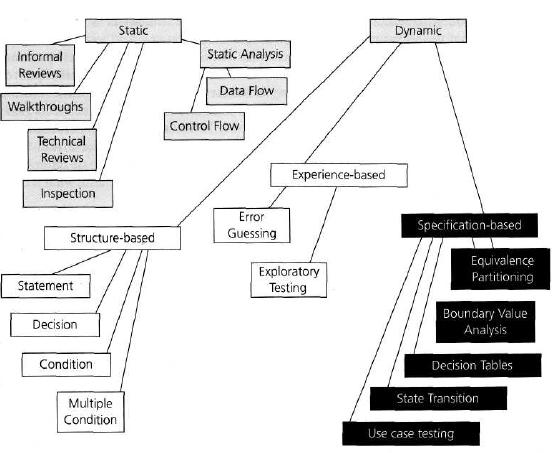
\includegraphics[width=10cm,keepaspectratio]{mtran_ima_cuoi}}
\caption{Các kỹ thuật kiểm thử}
\label{fig:mtran_ima_cuoi}
\end{center}
\end{figure}
Có nhiều loại kỹ thuật kiểm thử phần mềm khác nhau, mỗi một loại đều có điểm mạnh và điểm yếu của nó. Phần toán rời rạc như chúng ta đã trình bày ở trên thì chủ yếu ứng dụng nhiều cho phần kiểm thử chức năng (phần in đậm trong hình \ref{fig:mtran_ima_cuoi}). Phần lý thuyết đồ thị ứng dụng nhiều trong phần kiểm thử cấu trúc. Dưới đây chúng ta sẽ tìm hiểu sơ bộ các loại đó và tìm hiểu xem vị thế của toán rời rạc sẽ nằm ở phần kiểm thử chức năng trong các kỹ thuật kiểm thử này.

\subsection {Các kỹ thuật kiểm thử tĩnh (Static testing techniques)}
Các kỹ thuật kiểm thử tĩnh không thực hiện kiểm tra bằng cách chạy mã (code) và thường được sử dụng trước khi kiểm thử được thực hiện trên phần mềm. Nó có thể được gọi là kỹ thuật không chạy code. Hầu hết các kỹ thuật kiểm thử tĩnh có thể được sử dụng để “kiểm thử” của bất kỳ hình thức của tài liệu bao gồm cả mã nguồn, tài liệu thiết kế và các mô hình, tài liệu kỹ thuật đặc tả chức năng và tài liệu đặc tả yêu cầu. Tuy nhiên  “phân tích tĩnh” là một loại công cụ hỗ trợ của kiểm thử tĩnh mà tập trung vào kiểm thử các ngôn ngữ hình thức và do đó thường dùng để kiểm thử tĩnh mà nguồn.

\subsection {Các kỹ thuật dựa trên tài liệu đặc tả kỹ thuật (black-box)}
Việc đầu tiên của kỹ thuật kiểm thử động chúng ta sẽ xem xét là dựa trên tài liệu đặc tả kỹ thuật. Đây cũng được gọi là “black-box” hoặc kiểm tra đầu vào/đầu ra bởi vì chúng ta xem xét các phần mềm như là như là một hộp đen (black-box) với đầu vào và đầu ra, nhưng họ không có kiến thức về hệ thống hoặc các thành phần cấu trúc bên trong hộp (box). Về bản chất, kiểm thử đang tâp trung vào phần mềm làm gì, và không tập trung vào nó làm thế nào.
Chú ý rằng định nghĩa này đề cập đến cả hai kiểm thử chức năng và không chức năng. Kiểm thử chức năng là có liên quan tới hệ thống này làm những gì, nó gồm tính năng hoặc chức năng. Kiểm thử phi chức năng liên quan đến hệ thống làm điều gì đó tốt như thế nào, hơn là hệ thống làm gì. Các khía cạnh phi chức năng (còn gọi là đặc tính chất lượng hoặc các thuộc tính chất lượng) bao gồm hiệu năng, khả năng sử dụng, tính khả chuyển, bảo trì, v...v. Các kỹ thuật kiểm thử phi chức năng ít thủ tục và ít chính thức chính thức hơn so với các loại khác như các bài kiểm thử thực tế có nhiều sự phụ thuộc vào loại hệ thống, nó làm gì và có sẵn cho các bài kiểm thử nguồn tài nguyên.
Kiểm thử phi chức năng là một phần của nghiên cứu và nó cũng được bao gồm trong \cite{istqb}. Có những kỹ thuật để phát sinh các kiểm thử phi chức năng [Gilb, 1988], [Các tiêu chuẩn kiểm thử], nhưn họ cũng không bao quát hết được ở mức cơ sở. Phân loại các kiểm thử hộp đen và hộp trắng được đề cập trong một số sách về kiểm thử, bao gồm [Beizer, 1990] và [Copeland, 2003].

\subsection {Các kỹ thuật dựa trên cấu trúc (white-box)}
Các kỹ thuật kiểm thử dựa trên cấu truc (kỹ thuật này cũng năng động hơn là kỹ thuật tĩnh) sử dụng cấu trúc bên trong của phần mềm để lấy các ca thử nghiệm. Chúng thường được gọi là “hộp trắng” (ngụ ý bạn có thể nhìn thấy hệ thống) kể họ yêu cầu các hiểu biết làm thế nào phần mềm được thực hiện, đó là phần mềm làm việc như thế nào. Ví dụ, một cấu trúc kỹ thuật có thể được quan tâm thực hiện các vòng lặp trong phần mềm. Các trường hợp thử nghiệm khác nhau có thể được bắt nguồn để thực hiện vòng lặp một lần, hai lần, và rất nhiều lần. Điều này có thể được thực hiện bất kể chức năng của phần mềm.

\subsection {Các kỹ thuật dựa trên kinh nghiệm}
Trong các kỹ thuật dựa trên kinh nghiệm, hiểu biết của mọi người, kỹ năng và kiến thức nền tảng là những đóng góp chính cho các điều kiện kiểm thử và các ca kiểm thử. Những kinh nghiệm của cả hiểu biết về kỹ thuật và nghiệp vụ là rất quan trọng, vì chúng mang lại những quan điểm khác nhau để phân tích kiểm thử và quá trình thiết kế. Do kinh nghiệm trước đó với hệ thống tương tự, họ có thể có cái nhìn vào những gì có thể không đúng, những gì là hữu ích cho kiểm thử.\\

Các kỹ thuật  dựa trên tài liệu đặc tả thích hợp ở các cấp thử nghiệm (thành phần kiểm tra thông qua để người sử dụng kiểm thử) trong đó tài liệu đặc tả tồn tại. Khi thực hiện hệ thống hoặc kiểm thử chấp nhận (acceptance testing), các tài liệu đặc tả yêu cầu hoặc đặc tả chức năng có thể là cơ sở cho các kiểm thử. Khi thực hiện thành phần hoặc kiểm thử tích hợp, một tài liệu thiết kế hoặc tài liệu đặc tả ở thức thấp là cơ sở cho các kiểm thử.
Kỹ thuật dựa trên cấu trúc cũng có thể được sử dụng ở mọi cấp độ thử nghiệm. Các lập trình viên sử dụng các kỹ thuật dựa trên cấu trúc trong thử nghiệm thành phần và thử nghiệm tích hợp các thành phần. Kỹ thuật dựa trên cấu trúc cũng được sử dụng trong hệ thống và kiểm thử chấp nhận.

Kỹ thuật dựa trên kinh nghiệm được sử dụng để bổ sung cho các kỹ thuật dựa trên tài liệu đặc tả và kỹ thuật dựa trên cấu trúc và cũng được sử dụng khi không có tài liệu đặc tả , hoặc các tài liệu đặc điểm nhưng không còn phù hợp hoặc đã lỗi thời. Điều này có thể là loại duy nhất của kỹ thuật được sử dụng cho các hệ thống rủi ro thấp, nhưng cách tiếp cận này có thể đặc biệt hữu ích dưới áp lực thời gian lớn - trong thực tế đây là một trong những yếu tố hàng đầu để kiểm thử thăm dò/khám phá.

%Phan tham chieu
\begin{thebibliography}{9}
\bibitem{istqb}
Dorothy Graham, Erik van Veenendaal, Isabel Evans, and Rex Black,
Foundations of software testing, ISTQB certification.
\bibitem{Lewis_fat_sv_vs_fat_client}
Lewis, T. and Evangelist,
Fat server vs fat clients: the transition from client-server to distributed computing,
American programmer, Vol. 7 No. 11, November 1994, pp.2-9
\bibitem{Milner_com_of_acm}
Milner, Robin,
Element of interaction (1993 Turing Award Lecture)
Communications of the ACM, Vol. 36, No. 1, January 1993.
\end{thebibliography}
% Ket thuc van ban
\end{document}
 
